% ------------------------------------------------------------------------
% file `6GT_phys2_ondes-exercise-18-exercise-body.tex'
%   in folder `xsim/'
%
%     exercise of type `exercise' with id `18'
%
% generated by the `exercise' environment of the
%   `xsim' package v0.21 (2022/02/12)
% from source `6GT_phys2_ondes' on 2024/05/31 on line 88
% ------------------------------------------------------------------------
    Un ukulélé \enquote{concert} a une longueur de corde d'environ 40cm, tandis qu'une guitare à une longueur de 64cm. On souhaite produire la même fondamentale sur ces deux instruments. Si on place la même corde sur les deux instruments, laquelle doit être la plus \enquote{tendue} ? Quel est le rapport entre les deux tensions ?
    \begin{figure}[ht!]
        \centering
        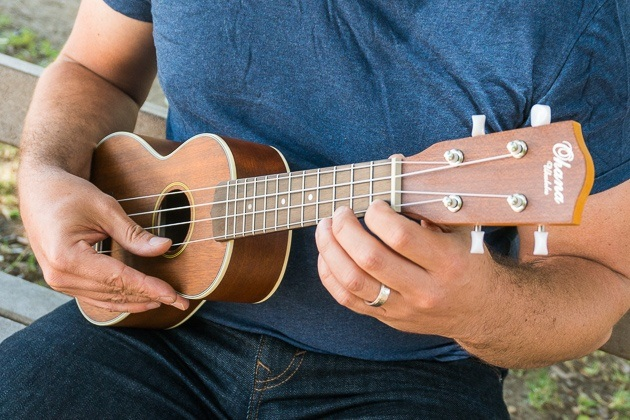
\includegraphics[width=.4\linewidth]{ukulele.png}
        \caption{Un ukulélé}
    \end{figure}
